\section{Problema 1: Laberinto}
\subsection{Introducción}

El escenario del primer problema es sencillo: dada una posición de arranque en un laberinto, queremos encontrar el camino mínimo hacia una posición final. Para lograr esto podemos derribar hasta cierta cantidad, ya determinada, de paredes del laberinto mismo. El input total del problema consiste de:

    \begin{itemize}
        \item Una matriz $M$ de caracteres que representan el mapa, de dimensión $F\times C$ (pasados por parámetro) donde $M_{ij} \in \{$'$\cdotp$'$,$'$\#$'$,$'$o$'$,$'$x$'$\}$ según sea, respecto del orden listado del conjunto, un lugar caminable, pared, punto de origen o punto de destino. Se asume que existe un único caracter $'o'$ y un único $'x'$ en todo el mapa.
        \item Un entero $P$ que representa la cantidad máxima de paredes que podremos romper, es decir, caracteres $'\#'$ que pueden conformar el camino mínimo cuya longitud buscamos.
    \end{itemize}

También sabemos por enunciado que los caracteres del borde del mapa corresponden a una pared. Lo que quiere decir que $i \in \{0, F-1\} \ \vee \ j \in \{0, C-1\} \Rightarrow M_{ij} =\ $'$\#$'.

Teniendo en cuenta que cada movimiento realizado debe ser vertical u horizontal (los vecinos de $M_{i,j}$ son los elementos en rango del conjunto $\{M_{i+1,j},\ M_{i-1,j},\ M_{i,j+1},\ M_{i,j-1}\}$), podemos considerar el output del problema como la mínima longitud de las secuencias válidas de vecinos en el mapa, empezando por el punto de origen (sin contarlo, dado que no es una ubicación a recorrer, sino que es la primer ubicación 'recorrida' del mapa) y terminando en el punto de destino, con cantidad de caracteres $'\#'$ menor o igual a $P$. La idea se formaliza como:
\\

    \begin{itemize}
        \item $ M_{ij} = $'$ o $'$ $
        \item $A = \Big\{ \langle {M_{i_0, j_0}\ ...\ M_{i_{k-1}, j_{k-1}}} \rangle \ \Big | \kern 0.2cm
        M_{i_0,j_0} \in \{M_{i+1,j}\ M_{i-1,j}\ M_{i,j+1}\ M_{i,j-1}\} \bigcap M_{[1..F]\times[1..C]} \kern 0.3cm \wedge \\ \sum\limits_{x=0}^{k-1} \beta(M_{i_x j_x} = $'$\#$'$) \leq P \kern 0.2cm \wedge \kern 0.2cm
        M_{i_{k-1}, j_{k-1}} = $'$\times$'$ \kern 0.3cm \wedge \kern 0.3cm
        \forall\ x \in [0..k-1) \kern 0.3cm M_{i_{(x+1)},j_{(x+1)}} \in \{M_{i_x+1,j_x}\\ M_{i_x-1,j_x}\ M_{i_x,j_x+1}\ M_{i_x,j_x-1}\} \bigcap M_{[1..F]\times[1..C]} \Big\}$
        \item $Output = \min\limits_{C \in A}\ |C|$
    \end{itemize}

Por ejemplo, sean los siguientes valores para $M$ y $P$:
\\
    \begin{center}
        $P=0, \kern 1cm
        M =
        \begin{bmatrix}
            \# & \# & \# & \# & \# \\
            \# & . & . & . & \# \\
            \# & \mathbf{o} & \# & \mathbf{x} & \# \\
            \# & . & . & . & \# \\
            \# & \# & \# & \# & \#
        \end{bmatrix}
        \kern 1cm
        (F = 5,\ C = 5)
        $

    \end{center}

Las secuencias de longitud mínima ($4$ en este caso) son los dos únicos caminos sin repetir ubicaciones: $\langle {M_{22}, M_{23}, M_{24}, M_{34}} \rangle$ y $\langle {M_{42}, M_{43}, M_{44}, M_{34}} \rangle$.

Para ilustrar un poco la idea del parámetro $P$ veamos también este caso:
\\
    \begin{center}
        $P=1, \kern 1cm
        M =
        \begin{bmatrix}
            \#  &   \#         &    \#    &   \#         &   \# & \#    \\
            \#  &   \mathbf{o}  &    \#     & \#          & \mathbf{x}    &   \#    \\
            \#  &   .         &    \#    &    .          &   .  & \#   \\
            \#  &   .          &    .     &   .          &   . & \#    \\
            \#  &   \#         &    \#    &   \#         &   \# & \#
        \end{bmatrix}
        \kern 1cm
        (F = 5,\ C = 6)
        $
    \end{center}

Si bien el camino más corto (obviando paredes) es $\langle {M_{23}, M_{24}, M_{25}} \rangle$, la suma de paredes atravesadas es $2 > P = 1$, por lo que tendremos que conformarnos la longitud $5$ del camino  $\langle {M_{32}, M_{33}, M_{34}, M_{35}, M_{25}} \rangle$
\\

El enunciado pide, además, una solución con complejidad $\mathcal{O}(FCP)$.

\subsection{Solución}

El enunciado pide abordar el problema desde una representación sobre grafos. Resulta bastante directo pensar cada nodo como el estado de nuestra ubicación en el mapa y cada arista como el movimiento hacia un vecino. Considerando también la restricción sobre $P$, es conveniente orientarlo en forma de digrafo (moviendonos podemos sumar demoliciones, pero no perderlas). Por lo tanto, nos interesaría encontrar algo similar al camino en dicho grafo que menos aristas contenga, considerando las siguientes modificaciones.

Sea $C \in M_{[1..F]\times[1..C]}$ una celda del mapa, la representamos con $P+1$ nodos de la pinta $ \langle {C,\ 0} \rangle ... \langle {C,\ P} \rangle$ donde $\langle $C,\ k$ \rangle$ representa el estado de haber llegado al casillero $C$ derribando exactamente $k$ paredes.

Si dos celdas $C_1$ y $C_2$ eran adyacentes en el mapa y $C_2$ es un espacio libre, $\langle {C_1,\ k} \rangle$ es adyacente a $\langle {C_2,\ k} \rangle$ para todo $k$, esto representa dar un paso desde $C_1$ hasta $C_2$ y, como no se destruyen paredes, se mantiene el contador de demoliciones. Si $C_2$ es una pared, entonces $\langle {C_1,\ k} \rangle$ será adyacente a $\langle {C_2,\ k+1} \rangle$ para todo $k < P$, representando el dar un paso desde $C_1$ a $C_2$ destruyendo la pared en el proceso. Si ya se habían destruido $P$ paredes, no es un paso válido destruir otra más.
Como nos interesa encontrar caminos mínimos (que pasen por la menor cantidad de aristas posibles), no podrá suceder que tras demoler una pared se vuelva a pasar por ella, ya demolida, porque entonces estaríamos dando \emph{al menos} dos pasos (uno para salir de la pared demolida y otra para volver a entrar) para volver a terminar en la misma casilla que ya estabamos. Si fuera un camino mínimo podríamos tomar el mismo camino pero sin la secuencia de salida y retorno a la casilla, y tendría longitud menor, lo cual es absurdo pues el camino anterior lo habíamos supuesto mínimo. Por lo tanto, solamente consideraremos caminos que no repitan nodos, es decir, caminos simples.
Al no repetir nodos en cada camino, cada vez que visitemos una pared será una demolición.

Nótese que algunos de los nodos podrían ser inalcanzables desde el punto de entrada, dependiendo de la disposición de las paredes en el mapa. Por ejemplo, no es posible alcanzar una pared con 0 demoliciones. En caso de que ninguno de los nodos de la casilla del punto de salida sea alcanzable, se retornará -1.
\\

El vértice  de inico al buscar el camíno será el correspondiente a la celda de inicio habiendo destruido 0 paredes y los vértices de llegada serán todos los correspondientes al casillero de llegada del mapa, ya que un camino puede llegar con cualquier cantidad entre 0 y $P$ de paredes destrudas y ser válido.

Este tipo de problemas se puede resolver de manera generalizada con variaciones de $BFS$ (\emph{breadth-first search}), que nos aseguran recorrer el grafo por niveles de 'profundidad' (o sea, distancia de la raíz, que sería nuestro punto de salida) y, por lo tanto, la primer solución que encontremos tendrá la misma o menor distancia al origen que cualquier otra. Esto se debe a que cada elemento se guarda en una estructura con organización \emph{'First In, First Out' (FIFO)}, y siempre estaremos visitando los estados del camino cuyo \emph{padre} haya sido visitado primero.

Vale mencionar también que, como las adyacencias del grafo se arman partiendo de las del mapa, no nos hace falta construir en memoria el grafo. Sino que vamos recorriendo usando la información de adyacencias del mapa.
\\

En este pequeño ejemplo podemos ver tanto la idea de la representación en grafo del problema como del tipo de iteración que realiza $BFS$:

    \begin{center}
        $P=1, \kern 1cm
        M =
        \begin{bmatrix}
            \# & \# & \# & \# & \# \\
            \# & . & . & . & \# \\
            \# & \mathbf{o} & \# & \mathbf{x} & \# \\
            \# & \# & \# & . & \# \\
            \# & \# & \# & \# & \#
        \end{bmatrix}
        \kern 1cm
        (F = 5,\ C = 5)
        $

    \end{center}


    \begin{figure}[H]
        \centering
        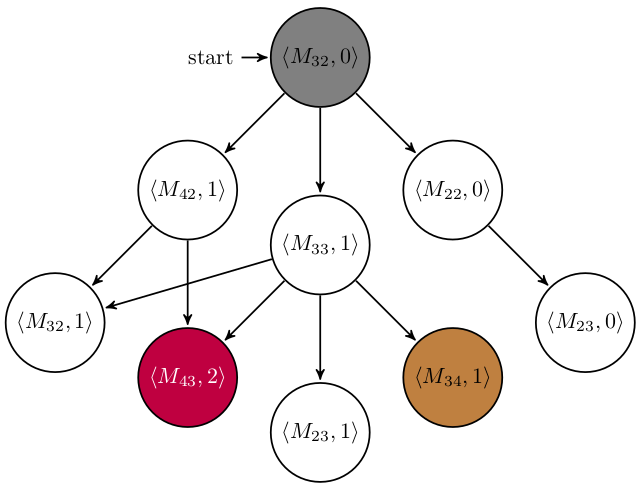
\includegraphics[width=12.0cm]{ej1-graph}
        \caption{El primer elemento de cada nodo revela la ubicación en el mapa y el segundo la cantidad de demoliciones contadas. Dependiendo del orden en que se desencolen los nodos padres, se definirán las ramas azules contra las verdes. El nodo rojo corresponde a un estado cuya rama, de seguir el algoritmo por no llegar ninguna rama al estado final en ese mismo nivel, sería podada. La longitud mínima de valor $2$ nos la da el camino $\langle {M_{33}, M_{34}} \rangle$. Como los puntos de arranque y de salida estarán en el interior del mapa (sino serían paredes), cada rama que pase por el borde tendrá que pasar por \emph{al menos} dos aristas más que la mínima dentro del mapa. Por lo tanto, por razones de espacio omitimos esas ramas en la figura (en el algoritmo sí se consideran). Además de que $P=1$ no permite recorrer el borde más que para salir del interior y luego volver al mismo nodo anterior, lo cual no podría ser mínimo.}
        \label{fig:ej1-graph}
    \end{figure}

    \begin{lstlisting}[caption={Pseudoc\'odigo de la resoluci\'on. En 'candidatos' se guardan los nodos tentativos que quedan por visitar. En dist se guarda la menor distancia que tienen al origen que, por iterar haciendo BFS, es la del primer camino en alcanzar dicho nodo.}]

        dist[m][n][p+1] $\leftarrow$ [m $\times$ n $\times$ (p+1)] * (-1)
        cola<<f, c>, k> candidatos

        dist[origen.f][origen.c][0] $\leftarrow$ 0
        candidatos.encolar(origen, 0)

        $\textbf{Mientras}$ $\neg$candidatos.vacio():
            actual $\leftarrow$ candidatos.desencolar()
            ubicacion $\leftarrow$ actual.first
            k $\leftarrow$ actual.second
            distancia $\leftarrow$ dist[ubicacion.f][ubicacion.c][k]

            $\textbf{Si}$ ubicacion = destino:
                $\textbf{Devolver}$ distancia

            $\textbf{Para cada}$ vecino <f,c> de ubicacion que este en rango:
                k_vecino $\leftarrow$ k + $\beta$(mapa[vecino.f][vecino.c] es pared)

                $\textbf{Si}$ k_vecino $\leq$ P $\wedge$ dist[vecino.f][vecino.c][k_vecino] $\neq$ -1:
                        candidatos.encolar(vecino, k_vecino)
                        dist[vecino.f][vecino.c][k_vecino] $\leftarrow$ distancia + 1

        $\textbf{Devolver}$ -1
    \end{lstlisting}


    Veamos que efectivamente el grafo modela bien el problema. En particular nos interesa ver que hay un mapeo directo entre los caminos simples del mapa (formalizados en la introducción a través de \emph{secuencias válidas de vecinos}, que además, como ya dijimos al presentar la representación del grafo, son los que formarán caminos mínimos) y los del grafo, y que además preserva su secuencia de ubicaciones y longitud final. De esta manera podremos aseverar que encontrar la longitud de un camino mínimo en el grafo es también encontrar la longitud de camino mínimo en el mapa porque existe alguno con esa longitud en él y, si hubiera otro con menor longitud, también lo habría en el grafo con la misma longitud (y por lo tanto el primero no era mínimo). Esto lo podemos formalizar en el siguiente lema:
    \\

    \begin{center}\textbf{\underline{Lema:} }\end{center}
        \textit{Para todo $M_{ij}$ en rango existe en el mapa un camino simple de distancia $n$ desde el punto de inicio $M_{s}$ y que además pasa por $k$ paredes si y sólo si existe un camino de $n$ aristas de distancia entre el vértice $\langle {M_s, 0} \rangle$ y el vértice $\langle {M_{ij},\ k} \rangle$  que recorre vértices asociados a las mismas ubicaciones (todas distintas) en el mismo orden.}
    \\

    Probemos el lema haciendo inducción en el largo $n$ de los caminos. Primero veamos la ida y luego la vuelta:

    \begin{center}$\mathbf{\implies}$\end{center}

    \textbf{\emph{Caso Base (n=1): }} Entonces $M_{ij}$ es vecino en el mapa de $M_s$ en el mapa. Si $M_{ij}$ es pared, entonces $k=1$, de lo contrario $k=0$ porque es el único punto que se visita desde el inicio. Por cómo construimos el grafo, $\langle {M_s, 0} \rangle$ y $\langle {M_{ij},\ k} \rangle$ son siempre adyacentes.
    \\

    \textbf{\emph{Paso inductivo (n$>$1): }} Supongamos un $M_{ij}$ en rango, con al menos un camino de longitud $n+1$ desde $M_s$ y $k$ demoliciones en él, quiero ver que existe algún camino de longitud $n$ entre $\langle {M_s, 0} \rangle$ y $\langle {M_{ij},\ k} \rangle$ donde la secuencia de primeras componentes de los vértices (todas distintas) coincide con el camino sobre el mapa.
    \\

    \emph{Hipótesis inductiva: } Como $n>1$, no son adyacentes y el camino tiene pasar por algún vecino $M_{xy}$ de $M_{ij}$ antes de terminar en este último. Por HI, a ese subcamino simple entre $M_s$ y $M_{xy}$ de longitud $n-1$ se le corresponde un camino entre $\langle {M_s,\ 0} \rangle$ y $\langle {M_{xy},\ k'} \rangle$ que pasa por las mismas ubicaciones. Como supusimos que el camino entre $M_s$ y $M_{ij}$ en el mapa tiene $k$ demoliciones podemos tomar, usando el mismo subcamino hasta su vecino, $k' = k - \beta(M_{ij}\ es\ pared)$. Esto se puede porque el camino que supusimos es simple, entonces $M_{ij}$ no fue visitado hasta el final y por lo tanto no está en el recorrido de $M_s$ a $M_{xy}$.

    Extendiendo el camino con la arista (existente por ser vecinos y construcción del grafo) entre $\langle M_{xy},\ k' \rangle$ y $\langle M_{ij},\ k''\rangle$ siendo $k'' = k' + \beta(M_{ij}\ es\ pared) = k$, nos queda un camino de longitud $n$ entre $\langle {M_s,\ 0} \rangle$ y $\langle {M_{ij},\ k} \rangle$ que recorre ubicaciones en el mismo orden que el supuesto al principio del paso inductivo. Además, como se corresponde con un camino simple, estas ubicaciones serán todas distintas entre ellas.
    \\

    \begin{center}$\mathbf{\impliedby}$\end{center}

    \textbf{\emph{Caso Base (n=1): }} Similar a la ida, por cómo armamos el grafo sabemos que existe un camino simple de $M_s$ a $M_{ij}$ con longitud 1 en el mapa porque sino $\langle {M_s, 0} \rangle$ y $\langle {M_{ij},\ k} \rangle$ no serían adyacentes en el grafo. Lo mismo para el valor de $k$, que es 0 si $M_{ij}$ no es pared, 1 de lo contrario.
    \\

    \textbf{\emph{Paso inductivo (n$>$1): }} Asumiendo $M_{ij}$ en rango tal que existe un camino que no repite ubicaciones entre vértices de longitud $n$ desde $\langle {M_s, 0} \rangle$ al vértice $\langle {M_{ij},\ k} \rangle$, quiero ver que hay un camino simple de longitud $n$ entre $M_{ij}$ y $M_s$, que pasa por $k$ paredes y las mismas ubicaciones.
    \\

    \emph{Hipótesis inductiva: } También como en la ida, podemos aprovechar que, por construcción y $n>1$, quitando la última arista que hace llegar el camino a $\langle {M_{ij},\ k} \rangle$, podemos formar un subcamino desde $\langle {M_s, 0} \rangle$ hacia algún vecino $\langle {M_{xy},\ k' } \rangle$,  $k'= k-\beta(M_{ij}\ es\ pared)$, de longitud $n-1$.

    Usando HI sobre el subcamino mencionado, sabemos de la existencia de un camino simple de longitud $n-1$ en el mapa que atraviesa $k'$ paredes y va desde $M_s$ hasta $M_{xy}$ recorriendo cada una de las ubicaciones indicadas por nuestro subcamino en el grafo. Y al existir una arista entre $\langle {M_{ij},\ k} \rangle$ y $\langle {M_{xy},\ k' } \rangle$ (tiene que existir por suposición del camino simple del paso inductivo), $M_{ij}$ y $M_{xy}$ son, por construcción del grafo, vecinos en el mapa.

    $M_{ij}$ no pertenece al camino desde $M_s$ hasta $M_{xy}$ que obtuvimos mediante la hipótesis inductiva, porque de hacerlo entonces el camino desde $\langle {M_{s},\ 0} \rangle$ a $\langle {M_{ij},\ k} \rangle$ de donde sale el subcamino sobre el que se aplica la HI tendría ubicaciones repetidas, en particular un vértice $\langle {M_{ij},\ k} \rangle$ y otro de la pinta $\langle {M_{ij},\ k''} \rangle$. Por lo tanto, podemos agregar la arista desde $M_{xy}$ a $M_{ij}$ al camino obtenido y tendríamos un camino simple de longitud $n$ desde $M_{s}$ a $M_{ij}$ con $k'+\beta(M_{ij}\ es\ pared) = k$ demoliciones.
    (al no pertenecer al camino hasta tu su vecino, la última arista se corresponde a un movimiento con demolición).
    \QEDB
    \\

\subsection{Complejidad}

    Previo a las iteraciones, hace falta inicializar la cola de candidatos (implementada con el tipo \href{http://www.cs.northwestern.edu/~riesbeck/programming/c++/stl-summary.html#queue}{\emph{queue}} de la STL de C++) y el arreglo multidimensional con las distancias (implementado con el tipo \href{http://www.cs.northwestern.edu/~riesbeck/programming/c++/stl-summary.html#vector}{\emph{vector}}, de manera anidada), lo cual cuesta  $\mathcal{O}(1)$ y  $\mathcal{O}(F\times C\times (P+1))$ respectivamente. Las dos inserciones correspondientes al origen se hacen en $\mathcal{O}(1)$.
    \\

    Consideraremos a la variable $n = F\times C\times (P+1)$ como la cantidad de estados posibles.

    Una vez iterando, tenemos una guarda en $\mathcal{O}(1)$ y todas las asignaciones y comparaciones que realizamos en el cuerpo también son $\mathcal{O}(1)$, realizadas $\mathcal{O}(estados) = \mathcal{O}(n)$ veces entendiendo que en peor caso vamos a desencolar todos los estados posibles (como se modifica su distancia al ser encolados, no es posible que vuelvan a evaluarse con distancia -1 y ser reencolados).
    \\

    Se evalúa una guarda que compara ubicaciones en $\mathcal{O}(1)$ al cuerpo de la cual se ingresa una única vez (en caso de haber solución) para retornar la distancia final.
    \\

    Por cada vecino del nodo actual, tendremos que verificar si está en rango y calcular si aumenta la cantidad de demoliciones. Ambas operaciones se hacen en $\mathcal{O}(1)$. Como cada estado tiene 4 vecinos (los correspondientes a moverse en las cuatro direcciones del mapa), esto sucederá $\mathcal{O}(estados) = \mathcal{O}(n) $ veces. Además, hay que actualizar la distancia para los vecinos que no hayan sido actualizados todavía ($\mathcal{O}(1)$ por cada vecino) y agregarlos a la cola de candidatos. La inserción en el tipo $queue$, por ser un \emph{container adaptor}, depende del contenedor sobre el cual se encuentre implementado pero tanto para vectores como para colas doblemente terminadas es $\mathcal{O}(1)$ amortizado. Asumiendo que todos los vecinos sean siempre vistos por primera vez, nos queda un total de $\mathcal{O}(n)$
    \\

    Sumando todas las complejidades, terminamos con una complejidad final de $\mathcal{O}(n)$ con $n = F\times C\times (P+1)$ y por lo tanto $\mathcal{O}(F\times C\times P)$ que, recapitulando, era nuestra complejidad temporal objetivo. 
